\documentclass{vldb}
\usepackage{graphicx}
\usepackage{balance}
\usepackage{url}
\usepackage{amssymb}

% COMANDO PER EVIDENZIARE PARTI DA LEGGERE ATTENTAMETE
\usepackage{color,comment}
\usepackage{soul}
\definecolor{lightcyan}{RGB}{210, 210, 250}
\newcommand{\hlc}[2][lightcyan]{{\sethlcolor{#1}\hl{#2}}}
%\newcommand{\hlc}{}

\usepackage{hyperref}
\hypersetup{pdftex,colorlinks=true,allcolors=blue}
\usepackage{hypcap}


\begin{document}

\title{E1: ENRON Sentiment}


\numberofauthors{2} 
\author{
\alignauthor
Andrea Jemmett\\
       \affaddr{Vrije Universiteit Amsterdam}\\
       \affaddr{Amsterdam, the Netherlands}\\
       \email{andreajemmett@gmail.com}
\alignauthor
Enrico Rotundo\\
       \affaddr{Vrije Universiteit Amsterdam}\\
       \affaddr{Amsterdam, the Netherlands}\\
       \email{enrico.rotundo@gmail.com}
}


\maketitle

\begin{abstract}
Email dataset analysis is a challenging task in terms of quantity and poor-structured data.
Anyway, the availability of big computational infrastructures such as cluster computers helps to face the former issue.
Indeed, such platforms provide high and scalable computing and unload the programmer from the burden of managing most of its parallelisation and distribution.
Unfortunately, email datasets usually come as unstructured dataset in the form of text files or, whenever they contain any markup structure, the actual data might not be well formed.
In that case, the data could be human-readable but hardly parsable by a machine.
Therefore, the analysis should include additional mining steps and many integrity checks, in order to minimise any possible inconsistencies.  

In the past years, several email datasets from diverse sources have been publicly released.
In this paper, we analyse the famous ``ENRON Corpus'' which contains 620k messages in about 150 mailboxes belonging to ENRON employees involved in a court case.
We extract and analyse sentiments within those messages using functional programming together with a well known engine for large-scale data processing. 
Thus, the analysis is run in a high performance computing cluster.   
We present our result as an interactive visualisation of the sentiment spread via emails together with the company's stock price of the same period.
\hlc{TODO: aggiungere le conclusioni!!!!!!!!!!!}

\end{abstract}


\section{Introduction}
Email is, at least on the user side, a simple mean of communication.
Its popularity is probably due to the simplicity of usage: users can send textual messages and attachments to other addresses, also from mobile devices~\cite{chen2002enterprise}.   
Thus, in the digital era it became very a popular way of communication between privates and companies.
Normally, corporate emails are characterised by a specific structure, for example \textit{user@company.com}, where the \textit{user} suffix is a mailbox identifier and \textit{company.com} is a distinguishable company web domain.
A corporate mailbox server can handle and store thousands of inbound or outbound messages every day, collecting quite a huge amount of exchanged data.

Email dataset analysis consists in analyse a dumped data in order to extract specific information (e.g., communication patterns, sentiment analysis, etc.).
Such analysis is expensive in terms of computation: the data is often composed of a multitude of items that have to be processed individually.
Therefore, such tasks are normally run in distributed environments which allow high degrees of parallelisation.
Cluster computing provides a platform for executing complex parallel tasks in a programmer-friendly environment~\cite{buyya1999high, zaharia2010spark, shvachko2010hadoop}.
This means the programmer does not explicitly code how to parallelise the computation.
Moreover, such systems rely on distributed file systems which provide large storage capabilities and support for redundancy and distributed accesses~\cite{weil2006ceph}.

Furthermore, email datasets usually come in a semi structured fashion in the sense that the actual data might not be well formed. 
For instance, recipients attributes and email's body can be difficult to parse.
Thus, the analysis should include some validation steps which increases the complexity of the whole analysis process.

In this paper, we present a sentiment analysis on the well-known ``ENRON Corpus'' which contains 619,446 messages over 158 users~\cite{shetty2004enron}.
This dataset has been published by the Federal Energy Regulatory Commission\footnote{\url{http://www.ferc.gov/}} during its early 2000s investigation on ENRON Corp. for bankrupt and fraud.
Although it contains the mailboxes of ENRON's employees which were involved in the court case, the messages include text from many more email addresses, for example personal or even external to the company.
We perform a sentiment analysis on that dataset using the state-of-the-art large-scale data processing tools.
Due to the size of the dataset, about 50GB, we need to parallelise the computation.
Thus, we use a functional programming language which is natively supported by Apache Spark engine.
The latter is deployed in a cluster system which runs the whole computation quickly and in a flexible distributed environment.

Our outcome is a visualisation of the sentiment extracted from employees' emails together with the ENRON's stock price of the same period.
\hlc{TODO: aggiungere le conclusioni!!!!!!!!!!!}

The rest of the paper is organised as follow.
Section~\ref{sec:r-w} introduces similar works and the kind of technology used in our work.
Section~\ref{sec:r-q} points out some research questions we try to answer by our analysis.
Section~\ref{sec:p-s} details our analysis setting with respect to the analysis pipeline and its technical architecture. 
Finally, Section~\ref{sec:exp} describes the of experiment run in order to collect our results and Section~\ref{sec:concl} draws some conclusion on the whole work.



\section{Related work}
\label{sec:r-w}
In this section we present an overview of some works related to this paper:
\textit{email dataset analysis}, \textit{sentiment extraction} from text and lastly \textit{large-scale data processing tools}.

\subsection{Email Dataset Analysis}
\label{sub-sec:email-dataset-analysis}
About email dataset analysis, literature reports many works focused on exploring, filtering and describing email datasets.
Datasets can be noisy and some preparatory work like filtering and reorganising might be helpful to have a better grip on the data.
For instance,~\cite{klimt2004introducing} provides metrics of the ``ENRON corpus'' as well as a description of it structure.
A thorough analysis of such structure highlights the presence of redundant and SPAM messages.
Similarly,~\cite{zhou2007strategies} describes some cleaning strategies for the aforementioned corpus.
In particular, the authors analyse the actual difficulties in cleaning a corporate email dataset which in the ENRON case are multiple and mainly related to the text-parsing phase.
Indeed, the authors claim there are a certain amount of duplicate emails, addresses and attachments which might come in a slightly different format, making the parsing more challenging.
For example, it is possible to identify duplicate messages by checking the MD5 digest of the email's body constrained by same day~\cite{corrada2004enron}.
Moreover, email bodies ofter report forwarded text or signatures which are not useful for a sentiment extraction.
The authors claim that within the ENRON dataset, only 250k messages are actually unique and they belong to a total of 149 employees.
In~\cite{klimt2004enron}, the authors investigate the feasibility of email folder prediction considering recipients attributes (e.g., \textit{From}, \textit{To}) as well as \textit{Subject} and \textit{body}.
Unfortunately, the F1-score achieved using a Support Vector Machine (SVM) seems very poor, ranging from $0.3$ to $0.7$. 


\subsection{Sentiment Extraction}
Sentiment extraction from text has been well studied in the past 10 years~\cite{aggarwal2012mining, das2007yahoo, bai2004sentiment, gamon2005pulse, bird2009natural}.
In~\cite{manning2014stanford}, the authors present a powerful deep-learning based tool for text annotation which provides sentiment labelling on a sentence-grain.
That tool is the state-of-the-art in text annotation and is distributed as a fast and easy-to-use Open Source library.
A live demo is also available on the related website\footnote{\url{http://nlp.stanford.edu:8080/sentiment/rntnDemo.html}}.
Most emails contain human written text, therefore it is likely to contain some kind of emotions.
Its spread is influenced by many factors (e.g., social, behavioural, etc.).
For example,~\cite{mohammad2011tracking} shows emotion patterns in email messages occur with different characteristics depending on the genders involved.
Specifically, the authors consider the eight basic and prototypical emotions~\cite{plutchik1980emotion} and point out their balance is biased depending on the gender of the sender/receiver genders.


\subsection{Large-scale Data Processing Tools}
In order to perform email dataset analysis it is often necessary to employ specific tools able to support large-scale data processing jobs.
Currently, there are many distributed tools available such as file systems and computing engines which often are shipped altogether as a single product~\cite{shvachko2010hadoop, zaharia2012resilient, meng2015mllib, shoro2015big, dean2008mapreduce, dean2010mapreduce}
The Hadoop Distributed File System (HDFS) provides reliable storage of very large datasets and it has been developed as Open Source version of the Google File System (GFS)~\cite{shvachko2010hadoop, ghemawat2003google}.
Altough HDFS is implemented in Java to support portability, it presents some performances drawbacks under certain conditions~\cite{shafer2010hadoop}.

MapReduce is a flexible data-processing tool that automatically parallelise map-reduce jobs over key/value pairs, it is usually deployed on a cluster of computers which can deliver sufficient performances speedup~\cite{dean2010mapreduce}.
This tools provides a powerful platform for deploying a diverse set of tasks.
For instance, most machine learning algorithms can be implemented as map-reduce tasks and therefore run over a MapReduce cluster~\cite{chu2007map}. 

Finally Apache Spark represents the state-of-the-art bundle which implement improved versions of the aforementioned functionalities~\cite{shoro2015big}.
Indeed, this tool has been designed in order to bundle multiple big-data functionalities and libraries (e.g., SQL, machine learning, graph analysis, etc.)~\cite{meng2015mllib}, as well as to boost the overall performance~\cite{gopalani2015comparing}.
Among many others, Spark provides advanced relational data processing which is close to traditional SQL databases systems~\cite{armbrust2015spark}. 


\section{Research questions}
\label{sec:r-q}
In this paper we show a sentiment analysis of an emails dataset.
Considering the ``ENRON corpus'' a lot of work has already been done (see Section~\ref{sub-sec:email-dataset-analysis}).
However, in order to give our contribution, we formalise the following research questions:
\begin{enumerate}
	\item Is it possible to extract useful and consistent sentiment information from a noisy dataset such as ``ENRON Corups''?
	\item Does the sentiment extracted from ENRON's emails correlate with the company's stock price of the same period?
	\item How individual behaviours affects the overall sentiment observable within a shoet (i.e., 1 day) timespan?
\end{enumerate}

In the rest of the paper we provide a description of our setting and we attempt to answer the research questions listed above.


\section{Project setup}
\label{sec:p-s}
In this section we explain our software setup and the developed architecture.
We created and deployed three Spark jobs, each one with a specific task, in
order to render them more easily maintainable, manageable and deployable.

\subsection{Archive Extraction}
\label{sub-sec:archive-extraction}
The first step in our data analysis pipeline comprises the extraction of the
dataset from its \textit{zipped} form. The dataset consists of a collection of
archives, each one enclosing an Enron's employee mailbox, containing emails in
both native (eml, pdf, docx) and plain text (in which attachments have been
converted into plain text too). We decided to extract and work with the plain
text messages, filtering out attachments. The \texttt{UnzipperDriver} job is
responsible for this. The goal of the job is to unzip the archives and store a
collection of Scala tuples of the kind \texttt{(mailboxName, documents)} where
the first element is the mailbox name (extracted from the zip filename) and
documents is a \texttt{Seq} of extracted documents.

\subsection{ETL}
\label{sub-sec:etl}
Second step is the \textit{ETL} (Extract, Transform, Load). Here the term
\textit{Extraction} has a different meaning than that of the previous job.
The extraction part in \texttt{ETLDriver} is about extracting data from emails
in a structured form, that is we need to extract emails body and headers from
the raw data. Do do this we created an \texttt{EmailParser} object that
implements the extraction and parsing logic. In this we apply a series of
transformations to the raw emails:
\begin{itemize}
	\item extract email headers (\textit{Date}, \textit{From}, \textit{To},
		\textit{Cc}, \textit{Bcc} and \textit{Subject});
	\item separate body from headers;
	\item clean body from common dataset footer \footnote{Every email contains a
		disclaimer from EDRM, the company that cleansed and published this
		version of the Enron Corpus};
	\item clean body from quoted emails, ``\textit{Original Message}'' and
		``\textit{Forwarded By}'' text and delimiters.
\end{itemize}

Because we are interested only in emails exchanged by Enron employees, we need a
way to retrieve and identify those people from the email headers. Unfortunately
this is not straightforward because addresses and people names have different
formats like ``\textit{first-name last-name}'', ``\textit{last-name, first-name}'',
``\textit{first-name last-name, email}'' or ``\textit{last-name, initial}''.
To solve this problem we use an external list of \textit{mailbox custodians}
that gives us first, last name and its role within Enron. We then search
\textit{From}, \textit{To}, \textit{Cc} and \textit{Bcc} headers for known
custodians. If for an email it fails to find any known custodian, the message is
discarded.

Next processing step consists in transforming the extracted dataset into a form
more easily manageable and queryable. We use CoreNLP to tokenize and find
sentiment at sentence level in emails. Because the sentiment is at sentence
level we need a way to aggregate those into a single sentiment for the whole
email. To aggregate sentiments we use the following formula:
\begin{equation}
	S = \frac{\sum_{s \in SS} s}{|SS|}
	\label{eq:sentiment-aggregation}
\end{equation}
where $SS$ is the set of sentence sentiments.

Last step consists in storing the dataset for future analysis. We split the
dataset in two: one contains the full email body and no sentiment, the other
does not contain the body but has sentiments. We do this in order to have a more
lightweight, sentiment-tagged corpus that we can analyse with more agility. We
convert both datasets into Spark SQL's \texttt{DataFrame} that enables us to
perform queries and data aggregation using the SQL language.

\subsection{Sentiment Analyser}
\label{sub-sec:sentiment-analyser}
Last job that we use in our pipeline is the \texttt{SentimentResumer}. It is
responsible for querying the sentiment-tagged dataset and joins it with Enron
stock prices based on date. To do this we group emails by date and then we
average the sentiments for that day and then join them with the stock prices
data on the date field. Lastly we store the results as JSON so that we can
then download them and use them for visualization purposes.

\subsection{Visualization}
\label{sub-sec:visualization}
The resulting JSON file is used to visualize the correlation of Enron stock
prices with email sentiment. We created a simple line chart with two lines and
two vertical axes. A line represents the stock prices and another represents
email sentiments. We built the interface in HTML and Coffeescript, using the d3
visualization library. Because the codebase is hosted on Github we have chosen
to deploy the visualization using Github Pages
\footnote{\url{http://acidghost.github.io/ENRON-sentiment-analysis/visualization/}}
which offers free hosting of static files.

\section{Experiment}
\label{sec:exp}
In this section we briefly explain the experiment run in order to obtain our results.
After running the setup described in Section~\ref{sec:p-s}, we collect the output data.
Then, we perform a post processing step in which we firstly resample the time series on a weekly (i.e., 7 days) basis using the average as aggregation function.
Moreover, we apply an interpolation function (i.e., polynomial, $4^{th}$ order) to smooth out our time series.
The result is shown in Figure~\ref{fig:sentiment_vs_stock} where we can notice the dramatic drop of the stock values by the end of 2001.
Although the sentiment value seems not to be strongly affected by the stock's drop, we point out it has a decreasing overall trend.
Indeed, the Pearson correlation  coefficient between the stock price and the sentiment time series is some $0.28$.

\begin{figure}[h!]
\centering
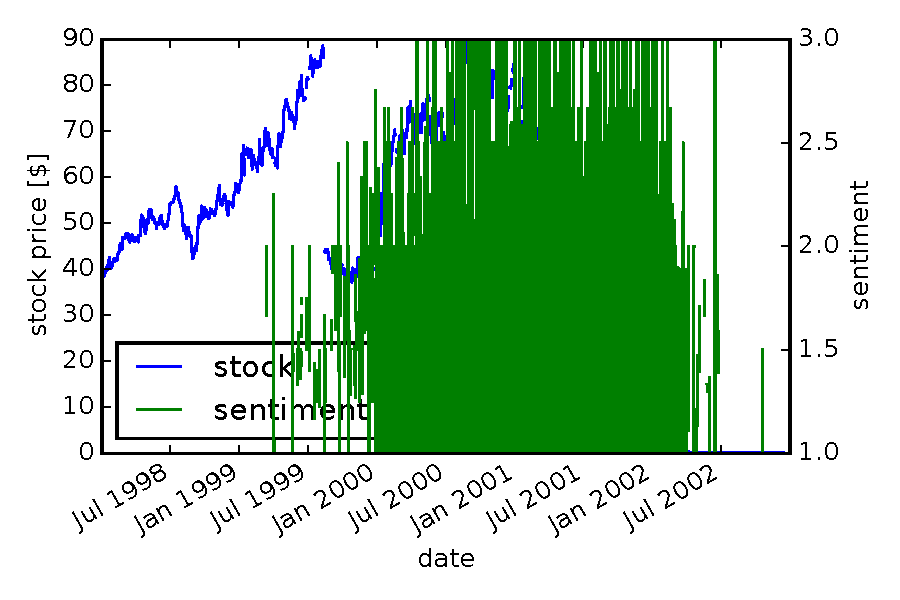
\includegraphics[width=0.48\textwidth]{imgs/sentiment_vs_stock}
\caption{Time series of ENRON's stock price (blue) and sentiment values extracted from emails (green), from 2000-01-01 to 2001-12-31.}
\label{fig:sentiment_vs_stock}
\end{figure}

Surprisingly, the distribution of sentiment values, shown in Figure~\ref{fig:sentiment_dist_hist}, does not show a significant standard deviation ($0.12$) over the considered time period.
This might be due to either low sentiment-annotation quality by the employed library, or most likely to some inconsistencies in the emails parsing task.

\begin{figure}[h!]
\centering
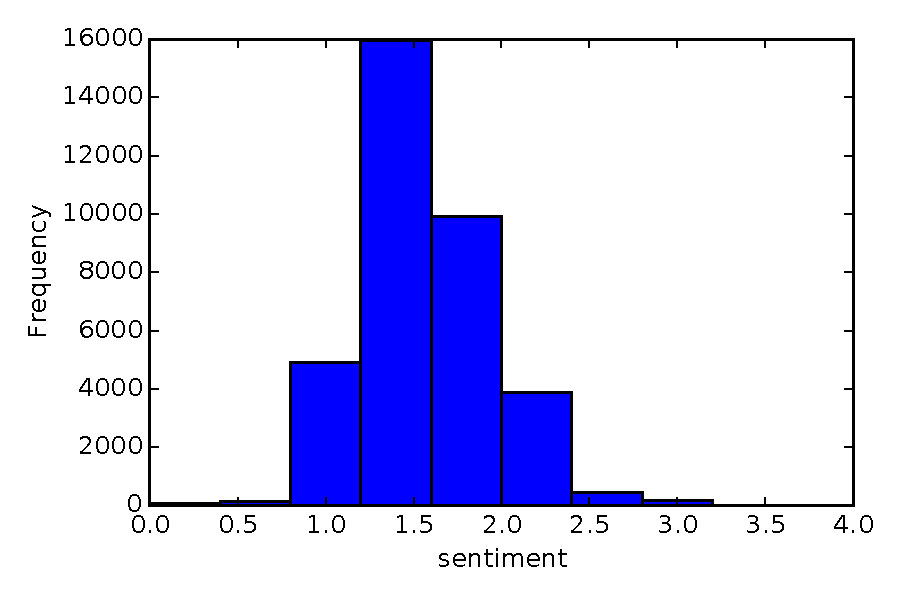
\includegraphics[width=0.48\textwidth]{imgs/sentiment_dist_hist}
\caption{Distribution of sentiment values extracted from emails, from 2000-01-01 to 2001-12-31.}
\label{fig:sentiment_dist_hist}
\end{figure}


\section{Conclusions}
\label{sec:concl}
In this section we present some conclusions based on our results, considering the research questions listed in Section~\ref{sec:r-q}.
Although, our results include a visualisation of sentiment information contained within the ``ENRON Corpus''.
Therefore, we claim the sentiment extraction from an emails dataset is actually doable. 
However, we highlight that in order to simplify our task we made some assumptions.
On one hand, we claim this is absolutely common, and sometimes even necessary, in a large-scale data processing.
On the other hand, the number and kind of assumptions might not be negligible.
For instance, we have chosen to take into account only those recipients which appears to have a personal mailbox in our dataset.
Therefore, people from outside the company and other employes are simply ignored.
Given that those people have most likely contributed to the sentiment coded in the emails, we argue this assumption is rather strict and further investigations should assess weather it is the case.  
\hlc{Furthermore, we claim that our visualisation provides useful hints for highlighting a not so strong correlation between emails' sentiment and the ENRON's stock price.
We argue this fact might be due to noise in our dataset,
Moreover, further experiments should be run with different settings, for example we could try different sentiment extraction techniques and other overall sentiment scoring functions.}
Lastly, we observe the research question about the influence of individual behaviours cannot find answer in this work.
This is mainly due to the lack of time to run further experiments.

As further conclusion, we would highlight some remarks on the usability of employed technologies.
In this paper we use Apache Spark which provides a distributed computing engine for running parallel applications.
Although this system is deployed in high performance cluster which provides large memory availability, the user is still in charge of estimating its memory needs and consequently to fine tune the memory allocation, also considering machines' physical limits.
Another highlight on Spark is the complexity of debugging some applications and the difficulty to read error logs.
Since user's applications are run over different machines, logs output are spread all over the cluster and users might suffer of not having direct and quick access to it.
 

\section{Acknowledgments}
We would like to remark our thankfulness to our teachers Peter Boncz and Hannes M{\"u}hleisen for their inspiration and support during this work and the LSDE 15-16 course held at Vrije Universiteit Amsterdam.
Last but not least we want to thank SURFsara\footnote{\url{www.surf.nl}} for providing the cluster computing platform necessary to run our experiments.

%\clearpage
%\balance
\bibliographystyle{abbrv}
\bibliography{bibliography} 

%\begin{appendix}
%TODO
%\section{BLA BLA}
%TODO
%\end{appendix}



\end{document}
